\documentclass[10pt,aspectratio=169]{beamer}
\usepackage{poly}
\usepackage{etoolbox}% new package to be loaded
\usepackage{amsmath,amssymb,amsthm}
\usepackage{tikz}
\usetikzlibrary{shapes.geometric, arrows.meta, positioning}

\AtBeginEnvironment{proposition}{% set of commands to be added
    \setbeamercolor{block title}{fg=white,bg=orange}% colors to change
    \setbeamercolor{block body}{fg=black}% colors to change
}
\AtBeginEnvironment{lemmas}{%
 \setbeamercolor{block title}{use=example text,fg=white,bg=blue!60!black!70}
  \setbeamercolor{block body}{parent=normal text,use=block title example,bg=block title example.bg!10!bg}

}
\AtBeginEnvironment{theorems}{%
 \setbeamercolor{block title}{fg=white,bg=red!70!black}
 \setbeamercolor{block body}{fg=black,bg=red!5}
}
\AtBeginEnvironment{corollarys}{%
 \setbeamercolor{block title}{fg=white,bg=green!50!black}
 \setbeamercolor{block body}{fg=black,bg=green!5}
}
% ================================================================================
% Metadata
% ================================================================================
%\title{On the Limitations of the Modulo Trick Method in Solving Exponential Diophantine Equations of the form $1+p^a=q^b+r^c$}
%\subtitle{Final Project Presentation}
%\author[Burapat, Kawin]{%
  %Mr. Burapat Suwanprasert (ID: 67983443) \\ 
  %Mr. Kawin Chumtong (ID: 67983115)
%}
%\institute{Assoc. Prof. Dr. Kijti Rodtes (Advisor)% \\ 
           %Science Classrooms in University-Affiliated School %Project (SCiUS) \\
           %Naresuan University Secondary Demonstration School}
%\date{February 26, 2026}

\title{On the Limitations of the Modulo Trick Method in Solving Exponential Diophantine Equations of the form $1+p^a=q^b+r^c$}
\subtitle{Final Project Presentation}
\author[Burapat, Kawin]{%
  Mr. Burapat Suwanprasert (ID: 67983443), Mr. Kawin Chumtong (ID: 67983115) 
}
\institute{Assoc. Prof. Dr.Kijti Rodtes (Advisor)}
\date{February, 26, 2026}

% ================================================================================
% Theorem Environments
% ================================================================================
\setbeamertemplate{theorems}[numbered]
\newtheorem{proposition}{Proposition}
\newtheorem{lemmas}{Lemma}
\newtheorem{theorems}{Theorem}
\newtheorem{corollarys}{Corollary}
\newtheorem{Definitionn}{Definition}
\newtheorem*{theoremss}{Theorem}

% ================================================================================
% Main Body
% ================================================================================
\begin{document}

% Title Slide
\maketitle

% Outline
\begin{frame}{Contents}
    \small
    \begin{tabular}{@{}p{0.82\linewidth}r@{}}
        Introduction & 3 \\
        Example from Brenner and Foster & 24 \\
        Understanding the Modulo Trick & 34 \\
        The Problem & 40 \\
        Objectives and Methodology & 45 \\
        Results & 47 \\
        \hspace{1em}Foundational Results & 47 \\
        \hspace{1em}Main Theorems & 54 \\
        \hspace{1em}Generalization & 62 \\
        Summary and Conclusion & 88 \\
    \end{tabular}
\end{frame}

% ================================================================================
% Section 1: Introduction with Storytelling Hook (Split Slides)
% ================================================================================
\section{Introduction}

\begin{frame}{Everyone Has Solved Equations, Right?}
    \begin{itemize}
        \item In school, we learn to solve many types of equations:
        \begin{itemize}
            \item \textbf{Linear equations:} $2x + 3 = 7$ \quad (Solution: $x = 2$)
            \item \textbf{Quadratic equations:} $x^2 - 5x + 6 = 0$ \quad (Solutions: $x = 2, 3$)
            \item \textbf{Systems of equations:} 
            $\begin{cases}
                2x + y = 5 \\
                x - y = 1
            \end{cases}$
        \end{itemize}
        \item These are familiar problems we've all encountered.
    \end{itemize}
\end{frame}

\begin{frame}{But What If We Restrict to Integers Only?}
    \begin{itemize}
        \item When we require solutions to be \textbf{integers}, we enter a different world.
        \item These are called \textbf{Diophantine equations}, named after Diophantus of Alexandria (3rd century AD).
        \item Example: $x^2 + y^2 = z^2$ has integer solutions: $(3,4,5)$, $(5,12,13)$, etc.
        \item Some equations that have real solutions may have \textbf{no integer solutions} at all!
    \end{itemize}
\end{frame}

\begin{frame}{Now, What If Unknowns Are in the Exponents?}
    \begin{itemize}
        \item This is where it gets really interesting. And we call it,
        \item \textbf{Exponential Diophantine equations:} Unknowns appear in the exponents.
        \item Example: $1 + 5^a = 7^b + 7^c$
        \begin{itemize}
            \item $a,b,c$ are unknown non-negative integers
            \item The bases $5,7,7$ are fixed
        \end{itemize}
        \item These equations are much harder to solve than polynomial equations.
        \item Our research focuses on the general form:
        \begin{equation}
            1+p^a = q^b + r^c \label{main}
        \end{equation}
        where $p,q,r$ are fixed positive integers.
    \end{itemize}
\end{frame}
\begin{frame}{If You Search on Google...}
    \begin{center}
        \fbox{\begin{minipage}{0.9\textwidth}
            \textbf{Google Search:} "exponential Diophantine equations"
        \end{minipage}}
    \end{center}
  
     
\end{frame}
\begin{frame}{If You Search on Google...}
    \begin{center}
        \fbox{\begin{minipage}{0.9\textwidth}
            \textbf{Google Search:} "exponential Diophantine equations"
        \end{minipage}}
    \end{center}
    \begin{figure}
        \centering
        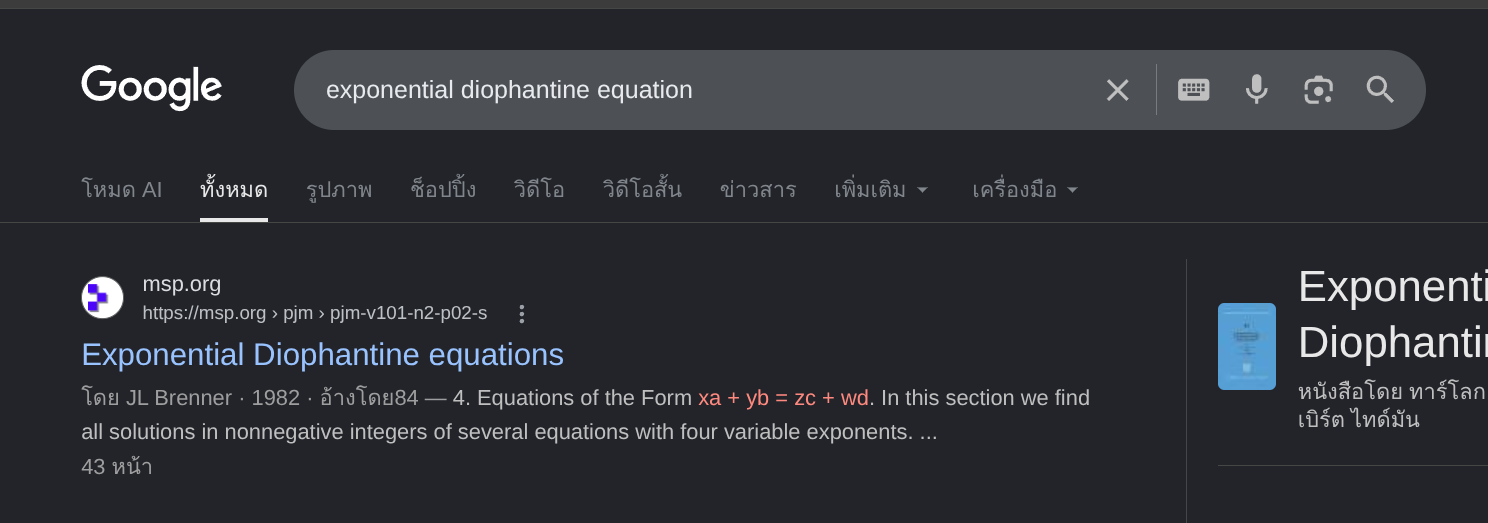
\includegraphics[width=0.7\linewidth]{image.png}
        \label{fig:placeholder}
    \end{figure}
    \begin{itemize}
        \item  \begin{block}{Brenner and Foster (1982)}
            "Exponential Diophantine Equations" \\
            \textit{Pacific Journal of Mathematics}, Vol. 101, No. 2, pp. 263-301
        \end{block}
    \end{itemize}
\end{frame}

\begin{frame}{Brenner and Foster's Paper}
        \begin{block}{Brenner and Foster (1982)}
            "Exponential Diophantine Equations" \\
            \textit{Pacific Journal of Mathematics}, Vol. 101, No. 2, pp. 263-301
        \end{block}
        This paper is all about:
        \begin{itemize}
            \item Solving several four-term exponential Diophantine equations
            \item  Including some cases of the form:
            \[1+p^a = q^b + r^c\]
            \item \textbf{Using an elementary method, especially the "Modulo trick" (Congruence method)}
        \end{itemize}
\end{frame}

% ================================================================================
% Section 2: Example from Brenner and Foster's Paper
% ================================================================================
\section{Example from Brenner and Foster}

\begin{frame}{Example from Brenner and Foster's Paper}
    \begin{block}{Equation 8.021 from their paper}
        \[1 + 5^a = 7^b + 7^c\]
    \end{block}
    
    \vspace{0.3cm}
    This is one of the equations they successfully solved using the modulo trick.
    
    \textbf{Why this example?}
    \begin{itemize}
        \item It's a concrete demonstration of how the method works
        \item Shows the step-by-step reasoning
        \item Illustrates the power of congruence methods
    \end{itemize}
    
    \vspace{0.2cm}
    Let's walk through their solution...
\end{frame}

\begin{frame}{Step 1: Set Up the Problem}
    We want to find all non-negative integers $(a,b,c)$ such that:
    \[1 + 5^a = 7^b + 7^c\]
    
    \vspace{0.3cm}
    \textbf{Observation:} The equation is symmetric in $b$ and $c$, so we can assume $b \leq c$ without loss of generality.
    
    \textbf{Strategy:} Use modular arithmetic to find constraints on $a$, $b$, and $c$.
\end{frame}

\begin{frame}{Step 2: Modulo 7 Analysis}
    Consider the equation modulo 7:
    \[1 + 5^a \equiv 7^b + 7^c \pmod 7\]
    
    Since $7^b \equiv 0 \pmod 7$ and $7^c \equiv 0 \pmod 7$ for $b,c \geq 1$:
    \[1 + 5^a \equiv 0 \pmod 7\]
    
    This means:
    \[5^a \equiv 6 \pmod 7\]
    
    \textbf{Question:} For which $a$ does $5^a \equiv 6 \pmod 7$?
\end{frame}

\begin{frame}{Step 3: Pattern of $5^a$ Modulo 7}
    Let's compute the pattern:
    
    \begin{tabular}{c|c}
        $a$ & $5^a \pmod 7$ \\ \hline
        1 & 5 \\
        2 & 4 \\
        3 & 6 \\
        4 & 2 \\
        5 & 3 \\
        6 & 1 \\
        7 & 5 \\
        8 & 4 \\
        9 & 6 \\
        $\vdots$ & $\vdots$
    \end{tabular}
    
    \vspace{0.2cm}
    \textbf{Pattern:} The sequence repeats every 6 steps.
    
    \textbf{Conclusion:} $5^a \equiv 6 \pmod 7$ when $a \equiv 3 \pmod 6$.
\end{frame}

\begin{frame}{Step 4: Modulo 9 Analysis}
    Now consider the equation modulo 9:
    \[1 + 5^a \equiv 7^b + 7^c \pmod 9\]
    
    First, find the pattern of $7^b$ modulo 9:
    
    \begin{tabular}{c|c}
        $b$ & $7^b \pmod 9$ \\ \hline
        1 & 7 \\
        2 & 4 \\
        3 & 1 \\
        4 & 7 \\
        5 & 4 \\
        6 & 1 \\
        $\vdots$ & $\vdots$
    \end{tabular}
    
    \vspace{0.2cm}
    So for $b \geq 1$, $7^b \in \{1,4,7\} \pmod 9$. For $b \geq 2$, we still have $7^b \in \{1,4,7\} \pmod 9$.
\end{frame}

\begin{frame}{Step 5: Compute $5^a$ Modulo 9 for $a \equiv 3 \pmod 6$}
    We know $a \equiv 3 \pmod 6$, so let's compute $5^a \pmod 9$:
    
    \begin{align*}
        5^3 &= 125 \equiv 8 \pmod 9 \\
        5^9 &= 5^{3+6} = 5^3 \cdot 5^6 \\
        5^6 &\equiv 1 \pmod 9 \text{ (by Euler's theorem)} \\
        \therefore 5^9 &\equiv 8 \cdot 1 = 8 \pmod 9
    \end{align*}
    
    In fact, for any $a \equiv 3 \pmod 6$, we have $5^a \equiv 8 \pmod 9$.
    
    Therefore:
    \[1 + 5^a \equiv 1 + 8 = 9 \equiv 0 \pmod 9\]
\end{frame}

\begin{frame}{Step 6: Compare Both Sides Modulo 9}
    We have:
    \begin{itemize}
        \item Left-hand side: $1 + 5^a \equiv 0 \pmod 9$
        \item Right-hand side: $7^b + 7^c \pmod 9$ where $7^b, 7^c \in \{1,4,7\}$
    \end{itemize}
    
    Check all possible sums:
    \begin{center}
    \begin{tabular}{c|c|c}
        $7^b$ & $7^c$ & Sum $\pmod 9$ \\ \hline
        1 & 1 & 2 \\
        1 & 4 & 5 \\
        1 & 7 & 8 \\
        4 & 4 & 8 \\
        4 & 7 & 2 \\
        7 & 7 & 5
    \end{tabular}
    \end{center}
    
    \textbf{None} of these sums equal $0 \pmod 9$!
    
    This is a contradiction unless our assumption was wrong.
\end{frame}

\begin{frame}{Step 7: Resolving the Contradiction}
    The contradiction arose because we assumed $b,c \geq 2$ when using modulo 9.
    
    Therefore, at least one of $b$ or $c$ must be $\leq 1$.
    
    \textbf{Possibilities:}
    \begin{itemize}
        \item $b = 0$ or $b = 1$
        \item $c = 0$ or $c = 1$
    \end{itemize}
    
    By symmetry, we only need to check a few cases:
    \begin{itemize}
        \item $(b,c) = (0,0)$, $(0,1)$, $(1,0)$, $(1,1)$
    \end{itemize}
\end{frame}

\begin{frame}{Step 8: Check the Remaining Cases}
    \textbf{Case 1:} $(b,c) = (0,0)$
    \begin{align*}
        1 + 5^a &= 1 + 1 = 2 \\
        5^a &= 1 \implies a = 0
    \end{align*}
    Solution: $(a,b,c) = (0,0,0)$
    
    \textbf{Case 2:} $(b,c) = (0,1)$
    \begin{align*}
        1 + 5^a &= 1 + 7 = 8 \\
        5^a &= 7 \implies \text{no solution}
    \end{align*}
    
    \textbf{Case 3:} $(b,c) = (1,0)$ (same as case 2 by symmetry)
    
    \textbf{Case 4:} $(b,c) = (1,1)$
    \begin{align*}
        1 + 5^a &= 7 + 7 = 14 \\
        5^a &= 13 \implies \text{no solution}
    \end{align*}
\end{frame}

\begin{frame}{Final Result from Brenner and Foster}
    \begin{theoremss}[Brenner and Foster, 1982]
        The only non-negative integer solution to
        \[1 + 5^a = 7^b + 7^c\]
        is $(a,b,c) = (0,0,0)$.
    \end{theoremss}
    
    \vspace{0.3cm}
    \textbf{Key insight:} The modulo trick worked because:
    \begin{itemize}
        \item Modulo 7 gave a condition on $a$
        \item Modulo 9 forced a contradiction unless $b$ or $c$ was small
        \item This gave an upper bound, making the equation computable
    \end{itemize}
    
    This is a perfect example of a successful application of the modulo trick.
\end{frame}

% ================================================================================
% Section 3: The Modulo Trick - Intuitive Introduction
% ================================================================================
\section{Understanding the Modulo Trick}

\begin{frame}{What is the Modulo Trick? An Intuitive Approach}
    \begin{itemize}
        \item Imagine you're trying to guess a number, but you can only ask questions about its remainder when divided by certain numbers.
        \item \textbf{Example:} I'm thinking of a number $x$. 
        \begin{itemize}
            \item If I tell you $x \equiv 1 \pmod 2$ (odd), what do you know?
            \item If I tell you $x \equiv 2 \pmod 3$, what do you know?
            \item Combining both, you can narrow down possibilities!
        \end{itemize}
        \item This is exactly what the modulo trick does - it uses remainders to restrict possible values of exponents.
    \end{itemize}
\end{frame}

\begin{frame}{The Basic Idea of the Modulo Trick}
    \begin{block}{Core Concept}
        Instead of solving $1+p^a = q^b + r^c$ directly, we ask:
        "What must be true about $a,b,c$ modulo different numbers?"
    \end{block}
    
    \vspace{0.3cm}
    \textbf{Why does this help?}
    \begin{itemize}
        \item Exponential expressions have predictable patterns modulo $m$
        \item By choosing the right moduli, we can force contradictions unless exponents are small
        \item Once exponents are bounded, we can check all remaining possibilities by brute force
    \end{itemize}
\end{frame}



\begin{frame}{How the Modulo Trick Works - Flowchart}
    \begin{figure}[h!]
        \centering
        \scalebox{0.5}{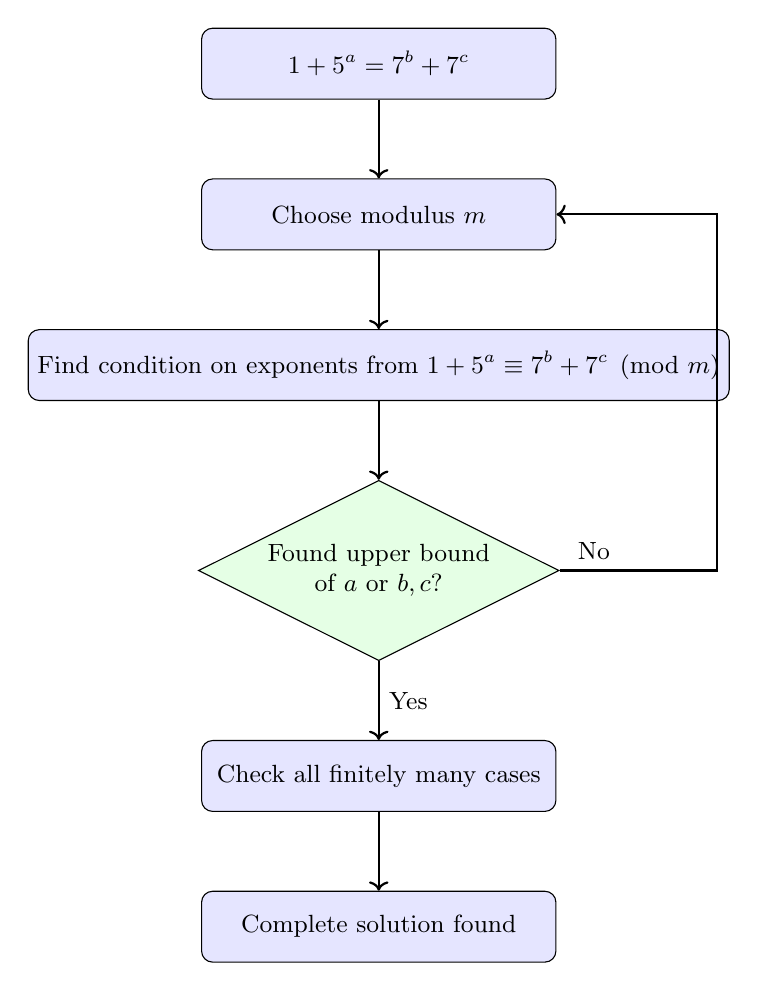
\begin{tikzpicture}[
            node distance=1cm,
            every node/.style={font=\small},
            box/.style={
                rectangle,
                draw,
                rounded corners,
                align=center,
                minimum width=4.5cm,
                minimum height=0.9cm,
                fill=blue!10
            },
            decision/.style={
                diamond,
                draw,
                align=center,
                aspect=2,
                inner sep=2pt,
                fill=green!10
            },
            arrow/.style={->, thick}
        ]
        
        % Nodes
        \node[box] (eq) {$1+5^a = 7^b + 7^c$};
        
        \node[box, below=of eq] (choosem) {Choose modulus $m$};
        
        \node[box, below=of choosem] (mod) {Find condition on exponents from $1+5^a \equiv 7^b+7^c \pmod m$};
        
        \node[decision, below=1cm of mod] (bound) {Found upper bound\\ of $a$ or $b,c$?};
        
        \node[box, below=of bound] (prop) {Check all finitely many cases};
        
        \node[box, below=of prop] (complete) {Complete solution found};
        
        % Arrows
        \draw[arrow] (eq) -- (choosem);
        \draw[arrow] (choosem) -- (mod);
        \draw[arrow] (mod) -- (bound);
        
        \draw[arrow] (bound) -- node[right] {Yes} (prop);
        \draw[arrow] (prop) -- (complete);
        
        % False loop
        \draw[arrow]
            (bound.east)
            -- node[pos=0.05, right, yshift=7pt] {No}
            ++(2,0)
            |- (choosem.east);
        
        \end{tikzpicture}}
        \caption{The modulo trick method applied to $1+5^a = 7^b+7^c$}
    \end{figure}
\end{frame}

\begin{frame}{Brenner and Foster's Success with Modulo Trick}
    Using the modulo trick, Brenner and Foster successfully solved many equations of the form $1+p^a = q^b + r^c$:
    
    \vspace{0.3cm}
    Examples they solved:
    \begin{itemize}
        \item $1+5^a = 7^b + 7^c$ (as we just saw)
        \item $1+2^a = 3^b + 5^c$
        \item $1+13^a = 17^b + 17^c$
        \item Many others with different base combinations
    \end{itemize}
    
    \vspace{0.3cm}
    The method worked well for these cases - they could always find some modulus that forced an upper bound on at least one variable.
\end{frame}

% ================================================================================
% Section 4: The Problem - Equations That Resist the Modulo Trick
% ================================================================================
\section{The Problem}

\begin{frame}{But They Found Equations That Resist the Method}
    Brenner and Foster encountered some equations that didn't yield to the modulo trick:
    
    \begin{quote}
        "The equations $(pq)^x - p^z - q^w + 1 = 0$ and $p^x - p^y + q^z - q^w = 0$ \textbf{seem not amenable} to our method."
    \end{quote}
    
    \vspace{0.3cm}
    In our form $1+p^a = q^b + r^c$, the first equation becomes:
    \[1 + (pq)^a = p^b + q^c\]
    
    \vspace{0.2cm}
    \textbf{They observed:} No matter which moduli they tried, they couldn't find upper bounds for the exponents. The method kept looping without ever reaching a contradiction.
\end{frame}

\begin{frame}{Why Do Some Equations Resist?}
    \begin{itemize}
        \item In our successful example $1+5^a = 7^b+7^c$, we found:
        \begin{itemize}
            \item Modulo 7 forced a condition on $a$
            \item Modulo 9 forced a contradiction unless $b$ or $c$ was small
        \end{itemize}
        
        \item For $1+(pq)^a = p^b+q^c$, something different happens:
        \begin{itemize}
            \item Modulo $p$: $1 \equiv 0 + q^c \pmod p$ gives condition on $c$
            \item Modulo $q$: $1 \equiv p^b + 0 \pmod q$ gives condition on $b$
            \item But these conditions don't create contradictions - they actually allow arbitrarily large solutions!
        \end{itemize}
        
        \item This suggests something fundamental: some equations are inherently immune to the modulo trick.
    \end{itemize}
\end{frame}

\begin{frame}{The Gap in the Literature}
    \textbf{What was missing}
    \begin{itemize}
        \item \textbf{Formal definition of solvable with modulo trick}
        \item \textbf{Rigorous reason some equations remain non-solvable}
        \item \textbf{Mathematical framework for the heuristic method}
    \end{itemize}

    \vspace{0.15cm}
    \textbf{Our research questions}
    \begin{enumerate}
        \item What does it \textbf{mean} for an equation to be "solvable by modulo trick"?
        \begin{itemize}
            \item \textbf{Short answer:} Repeated congruence checks leave only a bounded set of candidates.
        \end{itemize}
        \item Why are some equations "non-solvable" by this method?
        \begin{itemize}
            \item \textbf{Short answer:} Every finite modulus still leaves infinitely many unbounded candidates.
        \end{itemize}
        \item Can we \textbf{prove} the non-solvability of the cases Brenner and Foster observed?
        \begin{itemize}
            \item \textbf{Short answer:} Yes. We proved the main families and recovered their examples as corollaries.
        \end{itemize}
    \end{enumerate}
\end{frame}

% ================================================================================
% Section 5: Objectives and Methodology
% ================================================================================
\section{Objectives and Methodology}

\begin{frame}{Research Objectives}
    \begin{block}{Our goal}
        Turn the modulo trick from a useful idea into a precise method we can test, prove, and apply.
    \end{block}

    \vspace{0.15cm}
    \begin{columns}[T,onlytextwidth]
        \column{0.48\textwidth}
        \begin{exampleblock}{1. Define}
            \small Solvable and non-solvable by the modulo trick.
        \end{exampleblock}

        \begin{exampleblock}{2. Build}
            \small A simple framework for the method.
        \end{exampleblock}

        \column{0.48\textwidth}
        \begin{exampleblock}{3. Prove}
            \small When the method fails.
        \end{exampleblock}

        \begin{exampleblock}{4. Validate}
            \small Brenner and Foster observations.
        \end{exampleblock}
    \end{columns}
\end{frame}

\begin{frame}{Research Methodology}
    \begin{figure}[h!]
        \centering
        \scalebox{0.5}{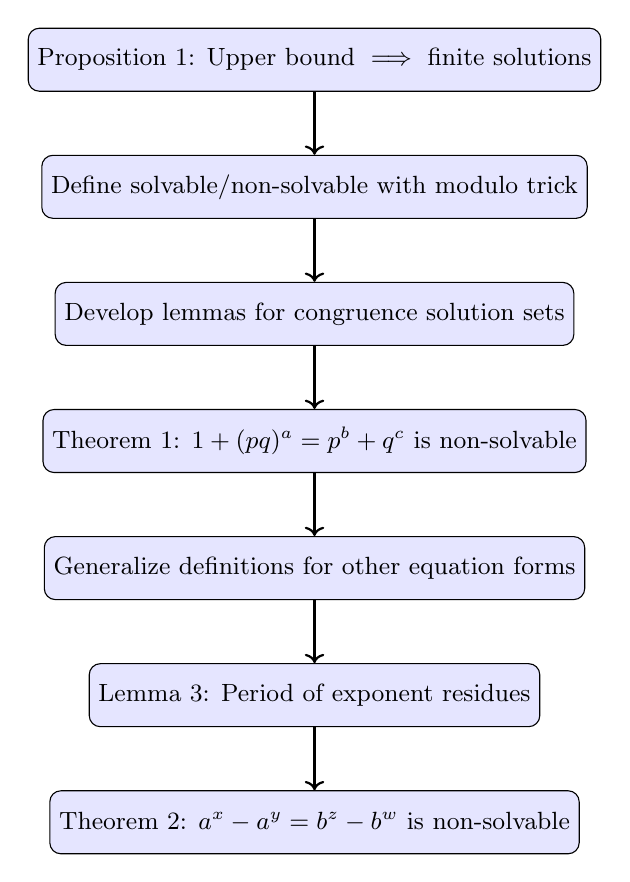
\begin{tikzpicture}[
            node distance=0.8cm,
            every node/.style={font=\small},
            box/.style={
                rectangle,
                draw,
                rounded corners,
                align=center,
                minimum width=4.5cm,
                minimum height=0.8cm,
                fill=blue!10
            },
            arrow/.style={->, thick}
        ]
        
        % Nodes
        \node[box] (1) {Proposition 1: Upper bound $\implies$ finite solutions};
        \node[box, below=of 1] (2) {Define solvable/non-solvable with modulo trick};
        \node[box, below=of 2] (3) {Develop lemmas for congruence solution sets};
        \node[box, below=of 3] (4) {Theorem 1: $1+(pq)^a = p^b+q^c$ is non-solvable};
        \node[box, below=of 4] (5) {Generalize definitions for other equation forms};
        \node[box, below=of 5] (6) {Lemma 3: Period of exponent residues};
        \node[box, below=of 6] (7) {Theorem 2: $a^x-a^y = b^z-b^w$ is non-solvable};
        
        % Arrows
        \draw[arrow] (1) -- (2);
        \draw[arrow] (2) -- (3);
        \draw[arrow] (3) -- (4);
        \draw[arrow] (4) -- (5);
        \draw[arrow] (5) -- (6);
        \draw[arrow] (6) -- (7);
        
        \end{tikzpicture}}
        \caption{Research methodology flowchart}
    \end{figure}
\end{frame}

% ================================================================================
% Section 6: Results
% ================================================================================
\section{Results}

\subsection{Foundational Results}

\begin{frame}{Proposition 1 - Key Insight for Computability}
    \begin{proposition}
       Equation $1+p^a = q^b + r^c$ is computable if at least one of these conditions holds:
       \begin{enumerate}
           \item There exists $M$ such that $a \leq M$ for any solution $(a,b,c)$
           \item There exist $M_b, M_c$ such that $b \leq M_b$ and $c \leq M_c$ for any solution
       \end{enumerate}
    \end{proposition}
    
    \textbf{Proof sketch (Condition 1):}
    \begin{align*}
        q^b+r^c &= 1+p^a \\
        q^b &= 1+p^a - r^c \leq p^a \leq p^M \\
        \implies b &\leq \frac{M\ln p}{\ln q},\quad c \leq \frac{M\ln p}{\ln r}
    \end{align*}
    
    \textbf{Conclusion:} All solutions lie in a finite set, hence computable in finite time.
\end{frame}
\begin{frame}{Modeling the Modulo Trick with Sets}
    \begin{block}{What happens when we apply the modulo trick?}
        \begin{itemize}
            \item We start with \textbf{all possible} exponent triples $(a,b,c)$
            \item We choose a modulus $m_1$ and impose: $1+p^a \equiv q^b+r^c \pmod{m_1}$
            \item This eliminates triples that don't satisfy this congruence
            \item We repeat with $m_2, m_3, ...$ - each time further restricting the possibilities
        \end{itemize}
    \end{block}
    
    \vspace{0.3cm}
    \textbf{We can represent this mathematically:}
    \begin{align*}
        S_0^{p,q,r} &= \mathbb{Z}_{\geq 0}^3 \quad \text{(all possibilities)} \\
        S_1^{p,q,r} &= \{(a,b,c) \in S_0^{p,q,r} \; | \; 1+p^a \equiv q^b+r^c \pmod{m_1}\} \\
        S_2^{p,q,r} &= \{(a,b,c) \in S_1^{p,q,r} \; | \; 1+p^a \equiv q^b+r^c \pmod{m_2}\} \\
        &\vdots \\
        S_k^{p,q,r} &= \{(a,b,c) \in S_{k-1}^{p,q,r} \; | \; 1+p^a \equiv q^b+r^c \pmod{m_k}\}
    \end{align*}
\end{frame}

\begin{frame}{From Sets to Definition of Solvability}
    \begin{block}{Key observation}
        After applying all moduli $m_1,...,m_k$, the set $S_k^{p,q,r}$ contains \textbf{all potential solutions} that survive all congruence conditions.
    \end{block}
    
    \vspace{0.2cm}
    \textbf{Recall Proposition 1:} If we can bound $a$ (or bound both $b$ and $c$), then all variables are bounded and the equation becomes computable by brute force.
    
    \vspace{0.3cm}
    \textbf{Therefore, the modulo trick succeeds exactly when:}
    \begin{itemize}
        \item After some finite sequence of moduli, the set $S_k^{p,q,r}$ contains only triples where:
        \begin{enumerate}
            \item $a$ is bounded by some $M_a$, OR
            \item both $b$ and $c$ are bounded by some $M_b, M_c$ respectively
        \end{enumerate}
    \end{itemize}
    
    \vspace{0.2cm}
    This is precisely our definition of \textbf{solvable with modulo trick} - it directly captures what the method aims to achieve!
\end{frame}
\begin{frame}{Formal Definition of Modulo Trick Solvability}
    Let $m_1,m_2,...,m_k$ be the sequence of moduli used. Define:
    \[S_0^{p,q,r} = \mathbb{Z}_{\geq 0}^3\]
    \[S_i^{p,q,r} = \{(a,b,c)\in S_{i-1}^{p,q,r} \; | \; 1+p^a \equiv q^b+r^c \pmod{m_i}\}\]
    
    \begin{Definitionn}
        Equation \eqref{main} is \textbf{solvable with modulo trick} if $\exists$ finite moduli $m_1,...,m_k$ such that:
        \begin{itemize}
            \item $\exists M_a$ with $M_a \geq a$ for all $(a,b,c) \in S_k^{p,q,r}$, OR
            \item $\exists M_b,M_c$ with $M_b \geq b$ and $M_c \geq c$ for all $(a,b,c) \in S_k^{p,q,r}$
        \end{itemize}
    \end{Definitionn}
    
    \begin{Definitionn}
        Equation \eqref{main} is \textbf{non-solvable with modulo trick} if for any finite moduli $m_1,...,m_k$:
        \begin{itemize}
            \item $\forall M_a$, $\exists (a,b,c) \in S_k^{p,q,r}$ with $a > M_a$
            \item $\forall M_b,M_c$, $\exists (a,b,c) \in S_k^{p,q,r}$ with $b > M_b$ or $c > M_c$
        \end{itemize}
    \end{Definitionn}
\end{frame}
\begin{frame}{Key Lemma - Single modulus lemma}
    \begin{lemmas}
        Let $A_m = \{(a,b,c) \in \mathbb{Z}_{\geq 0}^3 \; | \; 1+p^a \equiv q^b+r^c \pmod{m}\}$.
        For any moduli $m_1,...,m_k$,
        \[S_k^{p,q,r} = \bigcap_{i=1}^k A_{m_i} = A_{\operatorname{lcm}(m_1,...,m_k)}\]
    \end{lemmas}
    
    \textbf{Significance:}
    \begin{itemize}
        \item Any sequence of modular restrictions reduces to a \textbf{single modulus} (the LCM)
        \item Simplifies analysis dramatically
        \item Allows us to prove non-solvability by considering arbitrary single modulus
    \end{itemize}
\end{frame}

\subsection{Main Theorems}

\begin{frame}{Theorem 1 - Non-solvability of $1+(pq)^a = p^b + q^c$}
    \begin{theorems}
        For fixed coprime positive integers $p,q$, the equation
        \[1+(pq)^a = p^b + q^c\]
        is non-solvable with modulo trick.
    \end{theorems}

    \textbf{Proof strategy:}
    \begin{enumerate}
        \item By Lemma 3, it suffices to show for \textbf{any} modulus $m$, $A_m$ contains arbitrarily large $a,b,c$
        \item Factor $m = \chi \cdot \Gamma \cdot \mathrm{Z}$ where:
            \begin{itemize}
                \item $\chi$ contains primes dividing $p$
                \item $\Gamma$ contains primes dividing $q$
                \item $\mathrm{Z}$ contains primes dividing neither
            \end{itemize}
        \item Construct solutions using Euler's theorem $a^{\phi(n)} \equiv 1 \pmod n$ when $\gcd(a,n)=1$
        \item Parameters can be arbitrarily large $\implies$ non-solvable
    \end{enumerate}
\end{frame}

\begin{frame}{Corollary 1 - Validating Brenner and Foster (8.037)}
    \begin{corollarys}
        For fixed distinct primes $p,q$, the equation
        \[1+(pq)^a = p^b + q^c\]
        is non-solvable with modulo trick.
    \end{corollarys}
    
    \vspace{0.3cm}
    \textbf{Significance:}
    \begin{itemize}
        \item This is exactly the case mentioned by Brenner and Foster
        \item They observed it "seems not amenable" to congruence methods
        \item We have now \textbf{proved} this observation rigorously
        \item Provides mathematical validation for their heuristic comment
    \end{itemize}
\end{frame}

\subsection{Generalization}
\begin{frame}{Moving Beyond the Specific Form}
    \begin{block}{So far we've focused on:}
        \[1+p^a = q^b + r^c\]
    \end{block}
    
    \begin{itemize}
        \item This is just ONE type of exponential Diophantine equation
        \item We want to analyze other forms like:
        \begin{align*}
            &p^x - p^y = q^z - q^w \quad \text{(Brenner \& Foster 8.033)}\\
            &(pq)^a - p^b - q^c + 1 = 0 \quad \text{(Brenner \& Foster 8.037)}
        \end{align*}
        
        \item \textbf{Significance:} To prove non-solvability for these cases, we need definitions that work for ANY exponential Diophantine equation
        
        \item \textbf{Generalization strategy:} Extend our framework to handle equations of the form:
        \[C_1 + \sum_{i=1}^n k_i a_i^{x_i} = C_2 + \sum_{j=1}^m l_j b_j^{y_j}\]
    \end{itemize}
\end{frame}

\begin{frame}{General Form of Exponential Diophantine Equation}
    \begin{definition}[General Form]
        Let $n,m \in \mathbb{Z}^{+}$, and $C_1, C_2 \in \mathbb{Z}_{\geq 0}$ and $k_i, a_i, l_j, b_j \in \mathbb{Z}^{+}$ for $i=1,2,..,n$ and $j=1,2,...,m$. 
        
        Consider the exponential Diophantine equation
        \begin{equation}
            C_1 + \sum_{i=1}^n k_i a_i^{x_i} = C_2 + \sum_{j=1}^m l_j b_j^{y_j} \label{general}
        \end{equation}
        where $x_1,x_2,..,x_n, y_1,y_2,..,y_m \in \mathbb{Z}_{\geq 0}$.
    \end{definition}
    
    \textbf{Examples rewritten in this form:}
    \begin{align*}
        1 + 5^a &= 7^b + 7^c \quad (C_1=1, n=1, k_1=1, a_1=5, C_2=0, m=2, l_1=l_2=1, b_1=b_2=7)\\
        p^x - p^y &= q^z - q^w \quad (C_1=0, n=2, k_1=1, k_2=-1, a_1=a_2=p, C_2=0, m=2, l_1=1, l_2=-1, b_1=b_2=q)
    \end{align*}
    
    \textbf{Significance:} This unified notation lets us treat all exponential Diophantine equations with the same mathematical tools, regardless of their specific structure.
\end{frame}

\begin{frame}{Generalized Computability Criterion}
    \begin{lemma}[General Computability]
        Equation \eqref{general} is computable if at least one of these conditions hold:
        \begin{enumerate}
            \item There exist positive integer $M$ such that $x_1, x_2, ..., x_n \leq M$ for any solution.
            \item There exist positive integer $M$ such that $y_1, y_2, ..., y_m \leq M$ for any solution.
        \end{enumerate}
    \end{lemma}
    
    \textbf{Significance of this lemma:}
    \begin{itemize}
        \item This generalizes Proposition 1 from our specific equation to ANY equation of form \eqref{general}
       
    \end{itemize}
\end{frame}

\begin{frame}{Generalized Solution Sets After Moduli}
    \begin{definition}[Solution Sets]
        Let $m_1, m_2, ..., m_k$ be the sequence of moduli used for the modulo trick. We define:
        
        \[S_0 = \mathbb{Z}_{\geq 0}^{n+m}\]
        
        and for each $j = 1,2,...,k$:
        
        \[S_j = \left\{(x_1, x_2,..., x_n, y_1, y_2,..., y_m) \in S_{j-1} \;\middle|\;
        C_1 + \sum_{i=1}^n k_i a_i^{x_i} \equiv C_2 + \sum_{i=1}^m l_i b_i^{y_i} \pmod{m_j} \right\}\]
    \end{definition}
    
    \textbf{Notation:} For any modulus $k$, define the congruence solution set:
    
    \[A'_k = \left\{(x_1,...,x_n,y_1,...,y_m) \in \mathbb{Z}_{\geq 0}^{n+m}  \; |  \; C_1 + \sum_{i=1}^n k_i a_i^{x_i} \equiv C_2 + \sum_{i=1}^m l_i b_i^{y_i} \pmod{k} \right\}\]
    
    \textbf{Significance:} $S_k$ represents all tuples that survive all congruence conditions after applying the modulo trick. Any true solution to the original equation must be contained in $S_k$.
\end{frame}

\begin{frame}{General Definition of Solvability with Modulo Trick}
    \begin{definition}[General Solvability]
        The exponential Diophantine equation of the form \eqref{general} is called \textbf{solvable with modulo trick} if there exists a finite sequence of moduli $m_1, m_2, ..., m_k \in \mathbb{Z}^{+}$ used for modulo trick such that one of these conditions holds:
        
        \begin{itemize}
            \item There exists an integer $M$ such that $M \geq x_1, x_2, ..., x_n$ for any $(x_1, x_2, ..., x_n, y_1, y_2, ..., y_m) \in S_k$.
            
            \item There exists an integer $M$ such that $M \geq y_1, y_2, ..., y_m$ for any $(x_1, x_2, ..., x_n, y_1, y_2, ..., y_m) \in S_k$.
        \end{itemize}
    \end{definition}
    
    \textbf{Significance of this definition:}
    \begin{itemize}
        \item Captures exactly what the modulo trick aims to achieve - bounding one side of the equation
        \item Therefore, only finitely many tuples remain to check - the equation becomes computable!
        \item This definition works for ANY equation of form \eqref{general}
    \end{itemize}
\end{frame}

\begin{frame}{General Definition of Non-solvability with Modulo Trick}
    \begin{definition}[General Non-solvability]
        The exponential Diophantine equation of the form \eqref{general} is called \textbf{non-solvable with modulo trick} if for each finite sequence of moduli $m_1, m_2, ..., m_k \in \mathbb{Z}^{+}$ used for modulo trick, the following conditions hold for every $N, M \in \mathbb{Z}^{+}$:
        
        \begin{itemize}
            \item There exists $(x_1, x_2, ..., x_n, y_1, y_2, ..., y_m) \in S_k$ such that $N < x_i$ for some $i = 1,2,...,n$.
            
            \item There exists $(x_1, x_2, ..., x_n, y_1, y_2, ..., y_m) \in S_k$ such that $M < y_i$ for some $i = 1,2,...,m$.
        \end{itemize}
    \end{definition}
    
    \textbf{Significance of this definition:}
    \begin{itemize}
        \item No matter which moduli we choose, we cannot force either side of the equation to be bounded
       
        \item This formalizes what Brenner and Foster meant by "not amenable" to their method
    \end{itemize}
\end{frame}


\begin{frame}{Key Lemma - Generalized Single modulus lemma}
    \begin{lemmas}
        For any moduli $m_1,...,m_k$,
        \[S_k = \bigcap_{i=1}^k A'_{m_i} = A'_{\operatorname{lcm}(m_1,...,m_k)}\]
    \end{lemmas}
    
    \textbf{Significance:}
    \begin{itemize}
    \item  Generalized of lemma 1
        \item Any sequence of modular restrictions reduces to a \textbf{single modulus} (the LCM)
        \item Allows us to prove non-solvability by considering arbitrary single modulus
    \end{itemize}
\end{frame}
\begin{frame}{Lemma 3 - Period of Exponent Residues}
    \begin{lemmas}
        Let $a,n$ be positive integers. The sequence $(a^x \bmod n)_{x=1}^\infty$ is eventually periodic.
        
        That is, $\exists$ non-negative integers $k,\epsilon$ such that
        \[a^x \equiv a^{x+\epsilon} \pmod n\]
        for all $x \geq k$.
    \end{lemmas}
    
    \textbf{Proof sketch:}
    \begin{itemize}
        \item Residues are in $\{0,1,...,n-1\}$ (finite set)
        \item By pigeonhole principle, some residue repeats: $a^i \equiv a^{i+\epsilon}$
        \item Multiply by $a^t$ to extend periodicity
        \item  \textbf{Key insight:} Exponents can grow while maintaining congruence patterns
    \end{itemize}
    
    
\end{frame}

\begin{frame}{Theorem 2 - Non-solvability of $a^x-a^y = b^z-b^w$}
    \begin{theorems}
        Let $a,b \in \mathbb{Z}^+$. The exponential Diophantine equation
        \[a^x - a^y = b^z - b^w\]
        is non-solvable with modulo trick.
    \end{theorems}
    
    \textbf{Proof sketch:}
    \begin{enumerate}
        \item For any modulus $d$, by Lemma 3, $\exists$ periods $\epsilon_a,\epsilon_b$ and starting points $k_a,k_b$
        \item For any $x \geq k_a$, $y \geq k_b$, 
            \[(x,\; x+N\epsilon_a,\; y,\; y+M\epsilon_b) \in A'_d\]
        \item $x+N\epsilon_a,\;y+M\epsilon_b $ are increasing for any positive integer $N,M$
        \item Thus arbitrarily large exponents exist in $A'_d$ for any $d$
        \item Therefore non-solvable by modulo trick
    \end{enumerate}
\end{frame}

\begin{frame}{Corollary 2 - Validating Brenner and Foster (8.033)}
    \begin{corollarys}
        For fixed distinct primes $p,q$, the equation
        \[p^x - p^y = q^z - q^w\]
        is non-solvable with modulo trick.
    \end{corollarys}
    
    \vspace{0.3cm}
    \textbf{Significance:}
    \begin{itemize}
        \item Validates Brenner and Foster's comment (8.033)
        \item They noted this equation "cannot be fully investigated by reducing it to congruences"
        \item Our proof shows why: residues become periodic, allowing arbitrarily large solutions to satisfy any congruence
    \end{itemize}
\end{frame}

% ================================================================================
% Section 7: Summary and Conclusion
% ================================================================================
\section{Summary and Conclusion}

\begin{frame}{Summary of Main Results}
    \begin{itemize}
        \item \textbf{Example from Brenner and Foster:} $1+5^a = 7^b+7^c$ solved successfully with modulo trick
        
        \item \textbf{Formal definitions:} First rigorous characterization of "solvable by modulo trick"
        
        \item \textbf{Lemma framework:} Any sequence of moduli $\equiv$ single modulus (LCM)
        
        \item \textbf{Theorem 1:} $1+(pq)^a = p^b+q^c$ is non-solvable for coprime $p,q$
        
        \item \textbf{Theorem 2:} $a^x-a^y = b^z-b^w$ is non-solvable for any positive $a,b$
        
        \item \textbf{Corollaries:} Validated Brenner and Foster's observations (8.033, 8.037)
    \end{itemize}
\end{frame}

\begin{frame}{Conclusion}
\begin{itemize}
    \item[] \begin{block}{What we accomplished}
        \begin{itemize}
            \item Showed a concrete example of successful modulo trick application from Brenner and Foster
            \item Bridged the gap between heuristic observation and rigorous proof
            \item Provided mathematical foundation for why some equations resist elementary methods
            \item Created diagnostic tool for researchers
        \end{itemize}
    \end{block}
    
    \item[] \begin{block}{Practical recommendation}
        If an equation has the form $1+(pq)^a = p^b+q^c$ or $a^x-a^y = b^z-b^w$:
        \begin{itemize}
            \item Do \textbf{not} waste time with the modulo trick
            \item Proceed directly to advanced methods (Baker's theory, linear forms in logarithms)
        \end{itemize}
    \end{block}
\end{itemize}

\end{frame}

\begin{frame}{Future Work}
    \begin{itemize}
        \item Find non-trivial equations that \textbf{are} solvable with modulo trick
        \item Develop complete characterization of solvability conditions
        \item Apply framework to other forms of exponential Diophantine equations
        \item Investigate connections to Baker's theory and linear forms in logarithms
    \end{itemize}
    
    \vspace{0.5cm}
    \textbf{Challenges encountered:}
    \begin{itemize}
        \item Finding general conditions for solvability proved difficult
        \item May require deeper mathematical knowledge than expected
    \end{itemize}
\end{frame}

\begin{frame}{Key References}
    \begin{thebibliography}{9}
        \bibitem{eDe} J. L. Brenner and L. L. Foster, "Exponential Diophantine equations," \textit{Pacific J. Math.}, vol. 101, no. 2, pp. 263-301, 1982.
        
        \bibitem{wang} L. Wang and R. Tijdeman, "Exponential Diophantine equations with four terms," \textit{Indag. Math.}, vol. 51, pp. 87-96, 1988.
        
        \bibitem{DEZE199247} M. Deze and R. Tijdeman, "Exponential Diophantine equations with four terms," \textit{Indagationes Mathematicae}, vol. 3, no. 1, pp. 47-57, 1992.
    \end{thebibliography}
\end{frame}

\begin{frame}{Acknowledgments}
    \Large
    \centering
    \begin{itemize}
        \item Assoc. Prof. Dr. Kijti Rodtes (Advisor)
        \item Science Classrooms in University-Affiliated School Project (SCiUS)
        \item Naresuan University Secondary Demonstration School
        \item Our families for their unwavering support
        \item Our friends at SCiUS for the wonderful environment
    \end{itemize}
\end{frame}

\begin{frame}
    \Huge
    \centering
    Thank you for your time
    
    \vspace{1cm}
    \Large
    Any question?
\end{frame}

\end{document}

